\chapter{Development View}
The placement of components into a system is not always the same as the diagram of the
Logical View. It might be possible that two programs make use of the same set of packages. 
The Development View shows how these packages/components are distributed among the system.
It also shows at which time the different subsystems have to be finished in order to
succeed in developing the system as a whole.


% De rest van de development viewpoint
\section{Information}
The development view on this system is nearly the same as the logical view,
but some of the components that form the final STIFF system have to be developed
as a part of UCIS.\\
 \\
The STIFF system will do many proposal calculations during a single day. If the product
information inside the database doesn't change very often (which is the case here), it
is useless to query the database at every calculation request for the same product data.
This is why we decided that the product data should be kept in memory of the STIFF system,
and only if the product data is changed, that the STIFF systems refresh their data with
the new product information. Because the actual amount of STIFF systems is never known
by UCIS, there has to be some functionality which can tell all the STIFF systems to update
their memory. This is done by the STIFF Notifier.\\
The STIFF Notifier, which is part of the STIFF system, has to be developed
as a part of the business logic of UCIS. The STIFF Notifier will receive a message from UCIS
when the product information is changed in the database. The Notifier now sends a broadcast 
message to all the STIFF systems to update their memory, and all the systems behind the
load-balancing mechanism receive the update message.\\
 \\
In figure \ref{fig:development_final} you can see the deployment of the components of 
UCIS and STIFF.

\begin{figure}[ht]
	\centering
		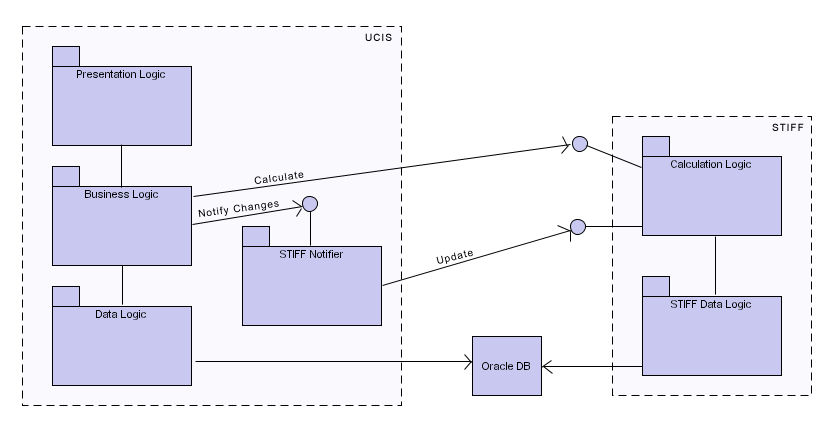
\includegraphics[width=1.00\textwidth]{img/development-final.png}
	\caption{Development View of UCIS and STIFF}
	\label{fig:development_final}
\end{figure}

\section{Evolution in time}
The time schedule in which the system has to be developed, can be shown best in the next Gantt 
diagram (see figure \ref{fig:gantt}). In the first phase, the system has to be altered in a way 
that it will perform direct requests (on demand) instead of batch-wise calculating the proposals.
To provide this functionality, both UCIS and STIFF have to be changed. UCIS will have some minor
changes, just the ones for benefiting of the real-time calculations of STIFF. STIFF on the 
other hand, will need some major refactoring to be done to ensure real-time calculations. The
whole system has to be transformed from Cobol into Java. Since this is too big of a step, we will
wait with the refactoring of STIFF until the third phase. In this first phase, STIFF will receive
a wrapper which starts the system on demand, and that just lets STIFF make use of its old components.\\
In this first phase, we also want to insert all the customer information of the customers of ForSure
into the Database of Zeker en Vast. Since the Oracle database isn't depending on ProD for storing
the actual insurances (the ProD doesn't keep track of pricing fluctuations for instance), 
the policies of the customers of ForSure can be added to the customer database without any problem.\\
 \\
In the second phase, the whole UCIS system will be refactored. It will get a new user interface
which will be accessible through the Internet, and all the business logic that had become part
of the client program will be put inside the main UCIS system again. Also, when the new GOC 
component is available, it will be added to the system in this phase. The last action in this
phase is to make sure the CHIPS and BuRP system make use of the new interfaces that will be 
provided in the new UCIS system.\\
 \\
In the third phase the STIFF system will be refactored. From now on, the STIFF system will be
totally scalable, and adding extra servers to provide more computational power will be very easy.
When STIFF is refactored, it will no longer make use of the old ProD database. All the product-data
will be stored in the main Oracle Database from this point on. When changes are made to the 
products, the STIFF systems will be automatically be notified by the UCIS system of that.


\begin{figure}[ht]
	\centering
		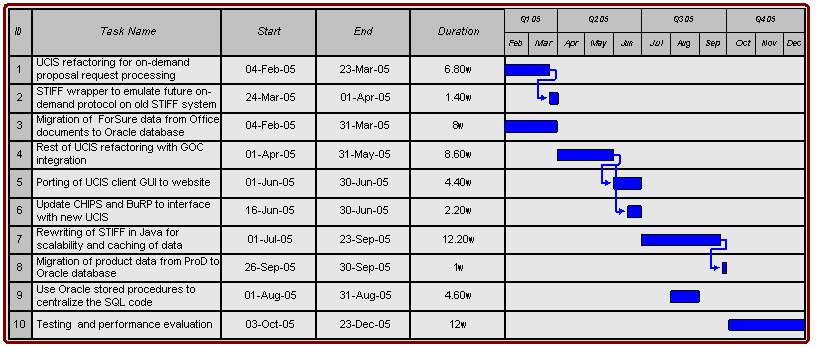
\includegraphics[width=1.00\textwidth]{img/gantt.png}
	\caption{Gantt diagram for the development of the system}
	\label{fig:gantt}
\end{figure}
